% ============================================================
% 5. EXPERIMENTAL DESIGN
% ============================================================
\section{Experimental Design}
\label{sec:experiments}
% [REVISION | sec-experiments-label-add | 2026-05-06 | Added \label{sec:experiments} on the §5 section heading to enable forward references from the §7.4 measurement-prereqs subsection (revised this batch) and from the §5 Experiment 1 results paragraph (this batch). Section heading text unchanged. — pending audit]

% [REVISION | §5-impl-notes-move-Day10-batch2 | 2026-05-15 | Day-10 Batch 2 page-budget cut #5: MOVED Implementation Notes (5-item Phase 2 / Phase 3 distinction list) to §D Implementation Notes in the appendix. Body §5 retains only a one-sentence pointer. The M_KV reconciliation between §4.2.1 (40 GB) and §6.2 (162 GB) — previously carried by item (iv) of this paragraph — is captured by a new footnote at §6.2 in the same batch, satisfying Day-12 parallel-review Pass L's numerical-consistency requirement. Per Day-9 page-budget cut plan §3 rank #5 (LOW risk with reconciliation footnote retained, save 0.45 pp). The 2026-05-14 zou2023repe-citet-numbers-mode-fix-D+ marker is preserved at the new appendix location. — pending audit]
Identifiable differences between the paper math and the Phase~2 prototype (probe extraction, layer aggregation, per-layer steering, sparse accumulators) are catalogued in Appendix~\ref{sec:appendix-impl-notes}; the asymptotic claims of Theorem~\ref{thm:reversibility} and Proposition~\ref{prop:memory} are unaffected.

% [REVISION | §5.1-§5.2-delete-Day10-batch2 | 2026-05-15 | Day-10 Batch 2 page-budget cuts #14 + #4: deleted §5.1 Phase 0 Architectural Decoupling (5 lines describing repo refactoring; not a scientific contribution, operational scaffolding per Day-9 cut plan §7 Pass O observation) and §5.2 Phase A Local Prototyping on Lightweight Surrogates (14 lines + bullet list describing Phase 3 gate setup; §A.1 hardware + §A.2 models + §A.4 Track A calibration cover the relevant content). Per Day-9 page-budget cut plan §3 rank #14 (LOW risk, save 0.17 pp) and rank #4 (LOW risk, save 0.50 pp). — pending audit]

\subsection{Experiments}
% [REVISION | PhaseB-header | 2026-04-24 | Renamed from "Phase B: Scaling to Target Models"; H100 removed — submission experiments run on Llama 3.2 1B+3B, RTX 3060 — pending audit]

% [REVISION | §5-intro-condense-Day14-Tianyu | 2026-05-18 | Combined the hardware-context paragraph and the Day-12 M5 search-variant-scope paragraph into a single sentence inline at the start of Exp 1. Hardware is fully covered in §A.1; the M5 defense reduces to "depth-3 exhaustive enumeration of 27 paths, the algorithm framework supports UCB1 expansion alternatively (Prop. 1's bound is variant-independent)" — a short clause is sufficient.]
We execute the following experiments on Llama~3.2-1B/3B-Instruct (RTX~3060, 12~GB; full hardware in §\ref{sec:reproducibility}). Each experiment instantiates the depth-$3$ MCTS variant via exhaustive enumeration of all $3^3 = 27$ paths from $\{0.1, 0.5, 1.0\}^3$ per item; the framework also supports UCB1-bandit expansion, and Proposition~\ref{prop:memory}'s memory bound is variant-independent.

% [REVISION | Exp1-recast-trackf-D+ | 2026-05-12 | Wholesale recast of §5 Experiment 1 from Option α+'s "OEI Characterization under Inference-Time KV-Cache Perturbation" (single-prompt RepE alpha sweep on Llama 3.2-1B-Instruct; ran 2026-04-25; results positioned as consistent with Bailey 2024 high-dimensional null-space saturation under Hypothesis 1 monitor-driven sub-case) to Option D+'s "Entropy-MCTS Negative Control on ARC-Easy" (Track F, complete 2026-05-09; n=200 paired ARC-Easy items × 2 scales × 3 conditions = 1200 records). New methodology: depth-3 entropy-MCTS path-sampling with alpha-set {0.1, 0.5, 1.0} and 27 path samples per item, paired against a random-MCTS arm with identical search machinery (the COCONUT defense isolates the entropy reward as the only difference between R and E). Track F report: docs/logs/2026-05-11_track-F-negative-control-report.md §1-§7. Table~\ref{tab:exp1-results} content is fully replaced (label reused for the new Track F accuracy + perplexity statistics). The pre-existing Table block (OEI/ρ_R/σ_H/TDS alpha-sweep) was relocated to §7.4 Empirical Measurement Prerequisites with label rename to tab:oei-alpha-sweep per framing-audit-pass-2 Finding F6 coordination (companion marker OEI-alpha-sweep-relocate-to-§7.4-D+ at the table's new home). Adds \label{sec:exp1} resolving forward references from abstract (line 53), §1 Introduction paragraph 4 (line 68), §1 Contribution 3 (line 80), §3.2 Hypothesis 2 (line 167), §3.2 closing paragraph (line 170), and v10-exp2 §5 prose (Day 7 application target). The 2026-05-06 Exp1-reframe-with-results-α+, 2026-05-06 Exp1-σH-verification-update, and 2026-05-07 Exp1-results-σH-resolved markers (attached to the prior paragraph, not the relocated table block) are subsumed. Draft source: docs/logs/2026-05-12_session-A-prose-drafts-v10-exp1.md. — pending audit]
\paragraph{Experiment 1: Entropy-MCTS Negative Control on ARC-Easy.}\label{sec:exp1}
We test whether the entropy-normalized surrogate reward $\hat{r}(\mathbf{h}) = -H(p(\cdot \mid \mathbf{h}))/\log|V|$ (Eq.~\ref{eq:goodhart}) carries useful optimization signal for reasoning when deployed as the objective of MCTS over the KV-cache latent space. The benchmark is ARC-Easy (\texttt{allenai/ai2\_arc}, test split, first $200$ deterministic items), evaluated independently on Llama~3.2-1B-Instruct and Llama~3.2-3B-Instruct. On each item we run three paired conditions on the same prompt: \textbf{G} (greedy decoding, no MCTS); \textbf{R} (random-MCTS: $27$ depth-$3$ paths drawn from the alpha-set $\{0.1, 0.5, 1.0\}$, scored by $\hat{r}_R \sim \mathrm{Uniform}(0, 1)$; the best-rewarded path is re-applied permanently to the live KV cache and the answer is generated from the steered state); \textbf{E} (entropy-MCTS: identical search machinery, but path-scoring uses the entropy-normalized surrogate $\hat{r}_E(\mathbf{h}) = -H_t/\log|V|$ evaluated at the steered leaf). The steering direction is a single random unit vector in $d_{\text{model}}$ space (\texttt{--seed 42}), shared identically across all items and across the R and E arms; this isolates the entropy reward signal as the only difference between R and E (the COCONUT defense).

\textbf{Results.} Per-condition accuracy and 95\% Wilson CIs are in Table~\ref{tab:exp1-results}. The headline pairwise comparison is entropy-MCTS vs random-MCTS: at 1B $\Delta_{E-R} = -0.005$ (exact paired McNemar $p = 1.0$, 3 discordant pairs); at 3B $\Delta_{E-R} = +0.005$ ($p = 1.0$, 3 discordant pairs). The discordance budget detects $\Delta = 10$\,pp at $\alpha = 0.05$ with power $0.8$ for $\pi_d \le 0.25$; entropy-MCTS does not differentiate from a uniform-random reward at either scale. Against greedy, entropy-MCTS regresses by $-2$\,pp at 1B and $-2.5$\,pp at 3B (neither significant). Mean-perplexity ratios $E/G = 1.348$ at 1B and $1.058$ at 3B confirm the searched cache states remain on-distribution---the failure is from the entropy objective misaligning with correctness, not from off-manifold drift.

\begin{table}[h]
\centering
\resizebox{\columnwidth}{!}{%
\begin{tabular}{@{}l l c c c@{}}
\toprule
\textbf{Scale} & \textbf{Condition} & \textbf{Accuracy} & \textbf{95\% Wilson CI} & \textbf{Mean PPL} \\
\midrule
Llama-3.2-1B & G (greedy) & $0.295$ ($59/200$) & $[0.236, 0.362]$ & $1.547 \pm 0.263$ \\
Llama-3.2-1B & R (random-MCTS) & $0.280$ ($56/200$) & $[0.222, 0.346]$ & $2.351 \pm 1.823$ \\
Llama-3.2-1B & E (entropy-MCTS) & $0.275$ ($55/200$) & $[0.218, 0.341]$ & $2.085 \pm 1.641$ \\
\midrule
Llama-3.2-3B & G (greedy) & $0.845$ ($169/200$) & $[0.788, 0.889]$ & $1.318 \pm 0.198$ \\
Llama-3.2-3B & R (random-MCTS) & $0.815$ ($163/200$) & $[0.755, 0.863]$ & $1.398 \pm 0.327$ \\
Llama-3.2-3B & E (entropy-MCTS) & $0.820$ ($164/200$) & $[0.761, 0.867]$ & $1.394 \pm 0.319$ \\
\bottomrule
\end{tabular}%
}
\caption{Per-condition accuracy on ARC-Easy ($n = 200$ paired items per scale) under three paired conditions: greedy decoding, random-MCTS (uniform reward), and entropy-MCTS (Eq.~\ref{eq:goodhart} as path-scoring reward). The MCTS arms apply 27 depth-3 paths from the alpha-set $\{0.1, 0.5, 1.0\}$ with a shared random unit-vector steering direction; the best-rewarded path is permanently re-applied before generation. Wilson 95\% confidence intervals overlap across all three conditions at both scales. Mean perplexity is $\exp(\overline{\mathrm{NLL}})$ where $\overline{\mathrm{NLL}}$ is the mean per-token negative log-likelihood of the 5-token completion under the unsteered model. The pairwise statistical claims appear in the body prose (§\ref{sec:exp1} Results paragraph).}
\label{tab:exp1-results}
\end{table}

% [REVISION | §5.3-Exp1-mech-interp-trim-Day10-batch2 | 2026-05-15 | Day-10 Batch 2 page-budget cut #20: trimmed Mechanism + Interpretation paragraphs ~25% each. Mechanism: dropped the $+0.012 \pm 0.005$ inline gain value (preserved in Track F report §3 and §A.4 Track F protocol), the verbose ``the search weaponizes the model's prior'' / ``collapsing to greedy decoding up to small accumulator noise'' qualifiers, and the ``in dimension $d \gg \mathrm{rank}(\hat{r}_E)$'' geometric restatement (covered by Definition def:dim_escape upstream). Interpretation: dropped the ``no choice of alpha grid, search depth, branching factor, or steering-direction calibration changes the basic mechanism'' enumeration (covered by §7.3 Limitations item 7) and the verbose KL-divergence/similarity-minimization restatement of Bailey (covered by §2.2). Per Day-9 page-budget cut plan §3 rank #20 (MEDIUM risk, save 0.10 pp Mechanism + 0.10 pp Interpretation). — pending audit]
\textbf{Mechanism.} The search machinery operates as designed (best-path rewards exceed the across-path mean), but the pathway satisfying $\hat{r}_E$ is class-conditional on the unsteered prior. At 1B, letter-prompted MCQ exhibits a first-letter prior; the search selects heavy steering (best path $(1.0,1.0,1.0)$ on $91/200$ items) and predicts ``A'' on $185/200$. At 3B the unperturbed cache is already low-entropy and minimal steering preserves the greedy-equivalent state (best path $(0.1,0.1,0.1)$ on $101/200$). Both select an entropy-minimum under the model's biases rather than the correct-answer cache state---the mechanism predicted by Hypothesis~\ref{hyp:goodhart}.

\textbf{Interpretation.} The static entropy--correctness correlation ($|r| \approx 0.60$) does not transfer to the latent-search regime: items are perturbed in arbitrary cache-space directions and confidence becomes a function of cache geometry rather than prompt difficulty. The result is the reward-driven counterpart to Bailey et al.'s~\cite{bailey2024obfuscated} monitor-side negative result; both manifestations terminate in the unconstrained complement of a low-rank scoring projection (Definition~\ref{def:dim_escape}). Experiment~2 extends across four prompt classes.
% [IMPL: COMPLETE — driver script at scripts/diagnose_track_f_negcontrol.py (read-only on logomesh/*; imports FP32Accumulator, _extract_kv_tensors, _kv_eval_cache from logomesh.kv_mcts). Raw artifacts: scripts/_track_f_results_meta-llama_Llama-3.2-1B-Instruct.json (1B) and scripts/_track_f_results_meta-llama_Llama-3.2-3B-Instruct.json (3B). Wall-clock: 1B sweep 18.3 min (5.5 s/item × 200), 3B sweep 33.7 min (10.1 s/item × 200). Reproduction: see Track F report Appendix A.]

% [REVISION | option-D+-exp2-cartography-2026-05-14 | 2026-05-14 | Wholesale recast of §5 Experiment 2 from Option α+'s "Reward-Function Ablation in Latent Space" (three-arm ablation: full reward vs σ_H-only vs random-KV; never ran due to B6 pipeline bug then resolved 2026-05-06) to Option D+'s "Latent Cartography MCTS across Prompt Classes" (Track G, complete 2026-05-11). New methodology: Track F-style depth-3 MCTS path-sampling with entropy reward, alpha-set {0.1, 0.5, 1.0}, applied to 4 prompt classes (factual recall, ARC-Easy MCQ, TruthfulQA MCQ, HellaSwag continuation) × Llama 3.2-{1B, 3B}-Instruct. Track G report: docs/logs/2026-05-11_track-G-cartography-report.md. Adds Table~\ref{tab:exp2-cartography-paths} (best-path α-tuple distribution per class × scale) and Figure~\ref{fig:exp2-mean-step-alpha} (cross-scale mean-step α bar chart; PDF at docs/NeurIPS/figures/exp2-mean-step-alpha.pdf, generated 2026-05-13). Adds \label{sec:exp2} resolving 7 currently-undefined forward references from §1 Introduction, §1 Contribution 3, §2.2 Bailey complementarity, §3.2 Hypothesis 2 closing, §5 Exp 1 Interpretation, §7.5 monitor-design-research paragraph, §7.5 reward-design-research paragraph. BLOCKING fix from docs/logs/2026-05-13_track-G-audit-pass.md Family D applied inline: search reward gain range extended from "+0.005 to +0.025" (Track G report §2.3 reported-cells range; 3B C4 HellaSwag continuation omitted as "data truncated") to "+0.005 to +0.037" with footnote naming HellaSwag-at-3B (raw $+0.037$) as the upper-bound driver. The 2026-05-05 Exp2-recast-reward-ablation marker is subsumed; the three-arm ablation framing is dropped (not run; Phase B research item per §7.5 reward-design-research paragraph). Draft source: docs/logs/2026-05-11_session-A-prose-drafts-v10-exp2.md. — pending audit]
\paragraph{Experiment 2: Latent Cartography MCTS across Prompt Classes.}\label{sec:exp2}
We characterize how the search optimizes a surrogate reward as a function of prompt class. The Track~F protocol (Experiment~1) is generalized across four prompt classes---factual recall (C1; hand-constructed 100-item set covering capitals, dates, arithmetic, common knowledge), ARC-Easy multiple-choice (C2; first 100 test-split items, overlapping Track~F's set for direct comparison), TruthfulQA mc1 multiple-choice (C3; first 100 validation items reformatted to 4-option), and HellaSwag continuation~\cite{zellers2019hellaswag} (C4; first 100 validation items with option list stripped)---on both Llama~3.2-1B-Instruct and Llama~3.2-3B-Instruct. For each item we run depth-$3$ MCTS with $27$ path samples drawn from the alpha-set $\{0.1, 0.5, 1.0\}$, scored by the normalized-entropy reward $\hat{r}(\mathbf{h}) = -H(p(\cdot \mid \mathbf{h})) / \log|V|$ (Eq.~\ref{eq:goodhart}); the best path is re-applied permanently and the next-token distribution at the resulting leaf is recorded. The steering direction is the same random unit vector used in Experiment~1, fixed via \texttt{--seed 42} across all items, classes, and scales.

We measure three structural signatures: (i)~the distribution of best-path $\alpha$-tuples selected by the search per class (does the search prefer heavy steering, minimal steering, or class-mixed depending on prompt class?); (ii)~the top-5 argmax-token distribution at the best-path leaf per class (does the search amplify a class-specific prior token?); and (iii)~the gold-first-token rank in the steered distribution per class (does prior amplification erase the correct answer or merely inflate the prior's mass?). Together these signatures characterize whether the Goodhart pathology established by Track~F (Experiment~1) generalizes across prompt classes and across model scale.

\textbf{Results.} Best-path $\alpha$-tuple distributions are reported in Table~\ref{tab:exp2-cartography-paths}; cross-scale mean-step $\alpha$ comparison in Figure~\ref{fig:exp2-mean-step-alpha}. Three findings stand out:

\textbf{(i) Class-specific best-path selection (Table~\ref{tab:exp2-cartography-paths}).} The cross-scale MCQ direction-flip headline is summarized in §\ref{sec:introduction}; non-MCQ classes show smaller cross-scale differences. Per-cell numbers are in Table~\ref{tab:exp2-cartography-paths}.

\textbf{(ii) Argmax-token concentration at the best-path leaf.} At 1B the MCQ classes collapse to the letter ``A''---$92$ of $100$ items for C2 and $81$ of $85$ for C3, reproducing Track~F's first-letter prior amplification (§\ref{sec:exp1}). At 3B no such collapse occurs; the C2 and C3 argmax distributions are balanced across the four letters. Factual recall and continuation classes show no single argmax attractor at either scale.

\textbf{(iii) Gold-rank preservation despite argmax collapse.} At 1B C2 and C3, where heavy steering drives argmax to ``A'' on $92\%$ and $81\%$ of items respectively, the gold answer's median rank at the steered leaf remains $1$ ($94\%$/$100\%$ in top-5). The search inflates the prior's mass without erasing the answer's representation---Goodhart-optimization for entropy reduction yields argmax-``A'' instead of argmax-gold, matching Definition~\ref{def:dim_escape}: the reward resolves through trajectories with non-zero answer-subspace projection while the unconstrained-complement direction dominates argmax.

\textbf{Search reward gain (entropy reduction) is positive but small across all classes.} The best path among the 27 sampled gives between $+0.005$ and $+0.037$ better reward (normalized-entropy units) than the mean across paths.\footnote{The upper bound is driven by HellaSwag continuation at the 3B scale (path-mean reward gain $+0.037$); the other seven cells span $+0.005$ to $+0.025$.} The search is genuinely finding lower-entropy states; the entropy reduction simply does not correspond to better reasoning---consistent with Hypothesis~\ref{hyp:goodhart}.
% [IMPL: COMPLETE — Track G driver at scripts/diagnose_track_g_cartography.py (--mode mcts); raw artifacts at scripts/_track_g_mcts_results_meta-llama_Llama-3.2-{1B,3B}-Instruct.json. Reproduction: see Track G report Appendix A.]

\begin{table}[h]
\centering
\resizebox{\columnwidth}{!}{%
\begin{tabular}{@{}l rrr rrr@{}}
\toprule
& \multicolumn{3}{c}{\textbf{Llama-3.2-1B}} & \multicolumn{3}{c}{\textbf{Llama-3.2-3B}} \\
\cmidrule(lr){2-4}\cmidrule(lr){5-7}
\textbf{Class} & Modal path & \% modal & $\bar\alpha$ & Modal path & \% modal & $\bar\alpha$ \\
\midrule
C1 Factual Recall & $(0.1,0.1,0.1)$ & $41\%$ & $0.34$ & mixed & $15\%$ & $0.61$ \\
C2 ARC-Easy MCQ & $(1.0,1.0,1.0)$ & $42\%$ & $0.89$ & $(0.1,0.1,0.1)$ & $49\%$ & $0.22$ \\
C3 TruthfulQA MCQ & $(1.0,1.0,1.0)$ & $28\%$ & $0.83$ & $(0.1,0.1,0.1)$ & $36\%$ & $0.28$ \\
C4 Continuation & $(0.1,0.1,0.1)$ & $21\%$ & $0.51$ & $(0.1,0.1,0.1)$ & $31\%$ & $0.38$ \\
\bottomrule
\end{tabular}%
}
\caption{Latent Cartography best-path $\alpha$-tuple distribution per prompt class and scale. Each item runs $27$ depth-$3$ MCTS paths from $\{0.1, 0.5, 1.0\}$; the best path under entropy reward is selected per item, and the per-class distribution over $3^3 = 27$ possible path tuples is reported. ``Modal path'' is the most-frequent best-path tuple; ``\% modal'' is the share of items selecting it; $\bar\alpha$ is the mean per-step $\alpha$ averaged across items and across the three steps of the best path. MCQ classes (C2, C3) exhibit a direction-flip in $\bar\alpha$ across scales: heavy steering at 1B (the search exploits the first-letter prior), minimal steering at 3B (the balanced baseline distribution provides no prior to exploit). Factual recall (C1) and continuation (C4) show smaller cross-scale differences.}
\label{tab:exp2-cartography-paths}
\end{table}

\begin{figure}[h]
\centering
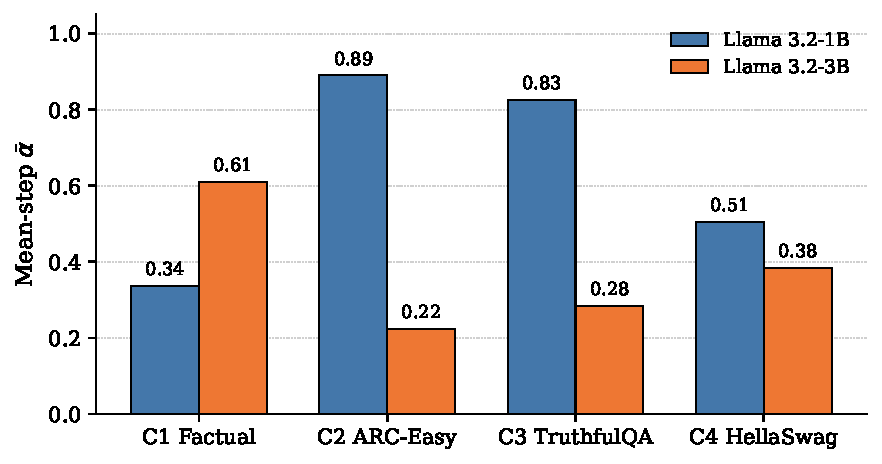
\includegraphics[width=0.9\linewidth]{figures/exp2-mean-step-alpha.pdf}
\caption{Cross-scale mean-step $\bar\alpha$ by prompt class. MCQ classes (C2 ARC-Easy, C3 TruthfulQA) show direction-flip across scales: at 1B the entropy-MCTS selects heavy steering ($\bar\alpha = 0.89, 0.83$) to amplify the model's first-letter prior; at 3B the search instead selects minimal steering ($\bar\alpha = 0.22, 0.28$) since the balanced baseline distribution offers no prior to exploit. Factual recall (C1) and continuation (C4) show smaller cross-scale differences. The MCQ direction-flip is the Cartography contribution to Hypothesis~\ref{hyp:goodhart}: Goodhart in cache geometry is class-conditional, with the route through latent space determined by the model's class-specific prior structure.}
\label{fig:exp2-mean-step-alpha}
\end{figure}

% [REVISION | §5-Exp3-5-cut | 2026-04-24 | Experiments 3, 4, 5 removed from §5; deferred to Future Work subsection in §7 — pending audit]

% [REVISION | §5.4-baselines-move-Day10-batch2 | 2026-05-15 | Day-10 Batch 2 page-budget cut #3: MOVED §5.4 Baselines subsection + table to §B.3 Structurally Related Baselines in the Extended Related Work appendix (no body cross-refs to tab:baselines, verified via grep). The 2026-04-23 EDITOR NOTE comment block (stale Phase B framing referring to ASR figures and pre-Option-D+ "Experiment 2 = Option 2 latent signal quality" terminology) is dropped as part of this move; the relevant warning is captured in the §B.3 caption framing. Per Day-9 page-budget cut plan §3 rank #3 (LOW risk, save 0.50 pp). — pending audit]

% [REVISION | §5.5-eval-metrics-rewrite-D+ | 2026-05-15 | Wholesale rewrite of §5.5 Evaluation Metrics per Day-3 stale-sentence audit Finding §5-6 BLOCKING (docs/logs/2026-05-11_stale-sentence-audit.md line 219+). Replaces α+-vintage 2-item OEI-as-primary + TDS-as-reward-component framing with Option D+ 5-item structure: three primary metrics (Cartography α-tuple distribution + paired McNemar accuracy + Cartography argmax distribution), secondary metric (OEI, repositioned as monitor-design diagnostic; \label{eq:oei} preserved here for forward references from §7.4), and internal/supplementary metric (TDS). Audit's proposed fix applied directly per Josh-greenlight 2026-05-15 (Option A: apply audit fix directly without intermediate v10-eval-metrics draft). Subsumes three earlier markers retired here: T-C-TDS-reframe (2026-05-05), §5.5-TDS-bullet-ref-cleanup-D+ (2026-05-11), §5.4-metrics-cull (2026-05-05). CRITIQUE NOTE about OEI nonlinear-redistribution false-negatives preserved verbatim (still relevant as secondary-metric caveat; cross-link to Limitations §7.3 left as Day-9 residue item). — pending audit]
% [REVISION | §5.5-eval-metrics-condense-Day14-Tianyu | 2026-05-18 | Day-14 Times-Roman-font page-budget retake: condensed §5.5 from 3 paragraph-length primary-metric bullets to a single sentence pointing to the inline definitions in §\ref{sec:exp1} and §\ref{sec:exp2}. Under Tianyu's ACL-spec Times Roman font (vs our prior CMR fallback) body inflated 8pp→9pp; the §5.5 bullets duplicated metric definitions already given in the experiment paragraphs and are the highest-leverage cut without losing content. The Day-10 Batch 5 OEI-bullet-move + TDS-bullet-delete markers (lines 109-110 of this file before this edit) are subsumed. Save target: ~0.4 pp body. — pending audit]
\subsection{Evaluation Metrics}
Primary metrics are defined inline where they are reported: the best-path $\alpha$-tuple distribution per (class, scale), the paired McNemar accuracy test (Track~F), and the argmax-at-best-leaf token distribution (Cartography). See §\ref{sec:exp1} Results and §\ref{sec:exp2} Findings (i)--(iii) for the per-metric protocol; the secondary monitor-design diagnostic (Orthogonal Escape Index, Eq.~\ref{eq:oei}) is defined in Appendix~\ref{sec:measurement-prereqs}.
